\documentclass{beamer}

% packages
\usepackage[utf8]{inputenc}
\usepackage[MeX]{polski}
\usepackage{hyperref}
\usepackage{colortbl}
\usepackage{graphicx}
\usepackage{pgfplots}
\usepackage{tikz, calc}
	\usetikzlibrary{arrows, shadings, shadows}
	\pgfplotsset{compat=1.8}

% theme
\usetheme{Ilmenau}
\definecolor{ios-top}{RGB}{30, 119, 239}
\definecolor{ios-bottom}{RGB}{129, 243, 254}
\definecolor{section-top}{RGB}{88, 86, 214}
\setbeamercolor{structure}{fg=ios-top}
\setbeamertemplate{blocks}[rounded][shadow=false, bg=red]
\setbeamercolor{block title}{bg=structure.fg!75!black}
\setbeamercolor{block body}{bg=structure.fg!30!white}
\setbeamertemplate{background canvas}[vertical shading][bottom=white,top=structure.fg!25]
\setbeamertemplate{sidebar canvas left}[horizontal shading][left=white!40!black,right=black]
\setbeamertemplate{itemize items}[triangle]
\setbeamercolor{section in head/foot}{fg=white,bg=structure.fg!75!black}
\setbeamercolor{alerted text}{fg=orange} 
\setbeamercolor{title in foot}{fg=white, bg=ios-top}
\setbeamertemplate{headline}
{%
  \begin{beamercolorbox}{section in head/foot}
  \vskip2pt\insertsectionnavigationhorizontal{\textwidth}{}{}\vskip2pt
  \end{beamercolorbox}
}
\setbeamertemplate{footline}
{%
  \leavevmode%
  \hbox{%
  \begin{beamercolorbox}[wd=.25\paperwidth,ht=2.25ex,dp=1ex,center]{author in head/foot}%
    \usebeamerfont{author in head/foot}\insertshortauthor
  \end{beamercolorbox}%
  \begin{beamercolorbox}[wd=.75\paperwidth,ht=2.25ex,dp=1ex,center]{title in foot}%
    \usebeamerfont{title in head/foot}\insertshorttitle\hspace*{3em}
    \insertframenumber{} / \inserttotalframenumber\hspace*{1ex}
  \end{beamercolorbox}}%
  \vskip0pt%
}
\setbeamertemplate{navigation symbols}{}

% author info 

\title[Mechanizm modelowania danych i mapowania obiektowego dla Apache Cassandry]{Praca Dyplomowa Magisterska}
\subtitle{Mechanizm modelowania danych i mapowania obiektowego dla Apache Cassandry}
\author[Jakub Turek]{Jakub Turek \\ {\small \href{mailto:J.Turek@stud.elka.pw.edu.pl}{J.Turek@stud.elka.pw.edu.pl}}}
\date{9 października 2014r.}

\begin{document}
	\begin{frame}
		\titlepage
	\end{frame}

	\section{Wstęp}

	\begin{frame}
		\frametitle{Cel pracy}

		System mapowania obiektowego dla bazy Apache Cassandra:

		\begin{itemize}
			\item Zachowanie różnicy w~wydajności pomiędzy relacyjnymi bazami danych a Cassandrą.
			\item Możliwość stosowania wzorców modelowania do optymalizacji.
			\item Zachowanie zgodności z istniejącymi mechanizmami mapowania obiektowo-relacyjnego.
		\end{itemize}
	\end{frame}

	\section{ORM}
	\subsection{Kundera}

	\begin{frame}
		\frametitle{Kundera}

		\begin{block}{Kundera}
			Implementacja Java Persistence API dla baz danych NoSQL.
		\end{block}

		\vspace{10pt}

		\begin{columns}[t]
			\column{.3\textwidth}
				Wspierane silniki:

				\begin{itemize}
					\item Cassandra
					\item HBase
					\item MongoDB
					\item Redis
					\item Oracle NoSQL
					\item Neo4j
					\item Couchdb
					\item Elastic Search
				\end{itemize}

			\column{.7\textwidth}
				Porównanie czasu wstawiania rekordów:

				\vspace{20pt}

				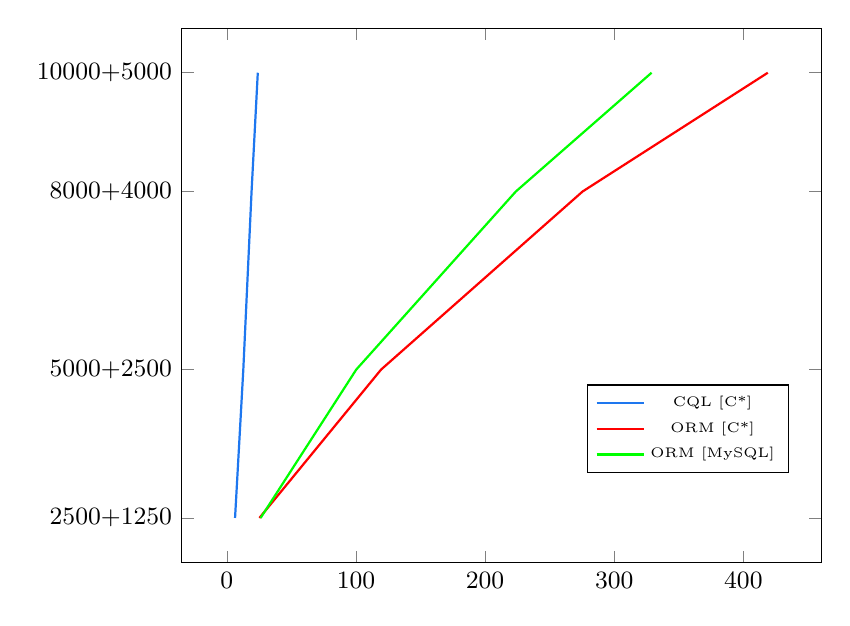
\begin{tikzpicture}
					\begin{axis}[
							width=.8\textwidth,
							scaled ticks=false, 
							tick label style={/pgf/number format/fixed},
							ytick={2500, 5000, 8000, 10000},
							yticklabels={2500+1250, 5000+2500, 8000+4000, 10000+5000},
							legend style={at={(0.95,0.25)},anchor=east,fill=none, font=\tiny},
							every axis/.append style={font=\small}
						]
						\addplot[color=ios-top, thick] coordinates {
							(23.978, 10000)
							(19.155, 8000)
							(12.762, 5000)
							(6.366, 2500)
						};
						\addlegendentry{CQL [C*]}

						\addplot[color=red, thick] coordinates {
							(418.915, 10000)
							(275.532, 8000)
							(119.453, 5000)
							(25.213, 2500)
						};
						\addlegendentry{ORM [C*]}

						\addplot[color=green, thick] coordinates {
							(328.915, 10000)
							(223.823, 8000)
							(100.23, 5000)
							(26.119, 2500)
						};
						\addlegendentry{ORM [MySQL]}
					\end{axis}
				\end{tikzpicture}
		\end{columns}
	\end{frame}

	\section{Zależności}

	\begin{frame}
		\frametitle{Analiza problemu}
		\framesubtitle{Modelowanie relacji wiele-do-wielu przez bibliotekę Kundera}

		\begin{columns}[c]
			\column{.5\textwidth}
				\scalebox{0.5}{
						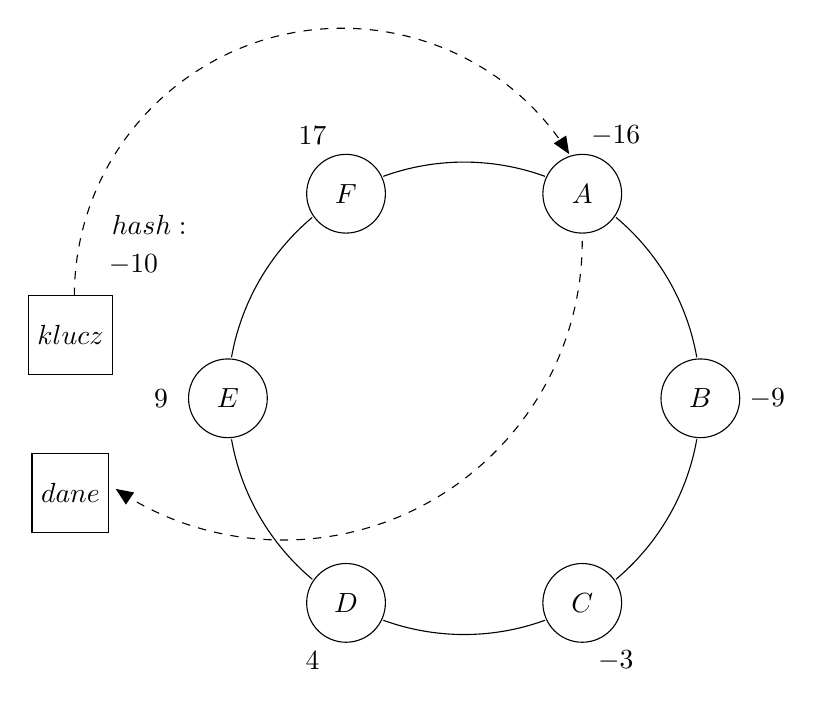
\begin{tikzpicture}
							\def \n {6}
							\def \radius {3cm}
							\def \margin {10}

							\foreach \a/\b [count=\s] in {B/-9, A/-16, F/17, E/9, D/4, C/-3}
							{
					  			\node[draw, circle, minimum width=1cm] at ({360/\n * (\s - 1)}:\radius) {$\a$};
					  			\node at ({360/\n * (\s - 1)}:3.85cm) {$\b$};
					  			\draw[>=latex] ({360/\n * (\s - 1)+\margin}:\radius) 
					    			arc ({360/\n * (\s - 1)+\margin}:{360/\n * (\s)-\margin}:\radius);
							}

							\node[draw, rectangle, minimum height=1cm] at (-5.0, 0.8) {$klucz$};
							\node[draw, rectangle, minimum height=1cm] at (-5.0, -1.2) {$dane$};
							\draw[dashed, -triangle 45] (-4.95,1.3) arc (180:32:3.4cm);
							\draw[dashed, -triangle 45] (1.5,2) arc (0:-124:3.8cm);
							\node at (-4.0, 2.2) {$hash:$};
							\node at (-4.2, 1.7) {$-10$};
						\end{tikzpicture}
				}

			\column{.5\textwidth}

				\begin{tabular}{l|l}
					\multicolumn{1}{c}{\textbf{Użytkownik}} & \textbf{Wiek} \\
					\hline
					\cellcolor{red!10}jkowalski & 24 \\
					\hline
					\cellcolor{red!10}mnowak & 45 \\
					\hline
				\end{tabular}

				\vspace{10pt}

				\begin{tabular}{l|l}
					\multicolumn{1}{c}{\textbf{Przedmiot}} & \textbf{Cena} \\
					\hline
					\cellcolor{red!10}laptop & 2276.99 \\
					\hline
					\cellcolor{red!10}audiobook & 42.40 \\
					\hline
				\end{tabular}
		\end{columns}

		\begin{center}
			\begin{tabular}{l|l|l|l}
				\multicolumn{1}{c}{\textbf{Klucz}} & \multicolumn{1}{c}{\textbf{Użytkownik}} & \multicolumn{1}{c}{\textbf{Przedmiot 1}} & \textbf{Przedmiot 2} \\
				\hline
				\cellcolor{red!10}1 & \cellcolor{yellow!10}jkowalski & \cellcolor{yellow!10}laptop & \cellcolor{yellow!10}audiobook \\
				\hline
				\cellcolor{red!10}2 & \cellcolor{yellow!10}mnowak & \cellcolor{yellow!10}audiobook & \cellcolor{yellow!10}\textit{(null)} \\
				\hline
			\end{tabular}
		\end{center}
	\end{frame}

	\begin{frame}
		\frametitle{Modelowanie zależności (1/2)}
		\framesubtitle{Zależność znormalizowana zwrotna}

		\begin{columns}[c]
			\column{.5\textwidth}

				\begin{center}
					\begin{tabular}{l|l}
						\multicolumn{1}{c}{\textbf{Użytkownik}} & \textbf{Wiek} \\
						\hline
						\cellcolor{red!10}jkowalski & 24 \\
						\hline
						\cellcolor{red!10}mnowak & 45 \\
						\hline
					\end{tabular}
				\end{center}

			\column{.5\textwidth}

				\begin{center}
					\begin{tabular}{l|l}
						\multicolumn{1}{c}{\textbf{Przedmiot}} & \textbf{Cena} \\
						\hline
						\cellcolor{red!10}laptop & 2276.99 \\
						\hline
						\cellcolor{red!10}audiobook & 42.40 \\
						\hline
					\end{tabular}
				\end{center}
		\end{columns}

		\begin{center}
			\begin{tabular}{l|l|l}
				\multicolumn{1}{c}{\textbf{Użytkownik}} & \multicolumn{1}{c}{\textbf{Przedmiot 1}} & \textbf{Przedmiot 2} \\
				\hline
				\cellcolor{red!10}jkowalski & laptop & audiobook \\
				\hline
				\cellcolor{red!10}mnowak & audiobook & \textit{(null)} \\
				\hline
			\end{tabular}
		\end{center}

		\begin{center}
			\begin{tabular}{l|l|l}
				\multicolumn{1}{c}{\textbf{Przedmiot}} & \multicolumn{1}{c}{\textbf{Użytkownik 1}} & \textbf{Użytkownik 2} \\
				\hline
				\cellcolor{red!10}audiobook & jkowalski & mnowak \\
				\hline
				\cellcolor{red!10}laptop & jkowalski & \textit{(null)} \\
				\hline
			\end{tabular}
		\end{center}
	\end{frame}

	\begin{frame}
		\frametitle{Modelowanie zależności (2/2)}
		\framesubtitle{Zależność zdenormalizowana zwrotna}

		\begin{center}
			\begin{tabular}{c|c|c|c|c|c}
				\multicolumn{1}{c}{\textbf{Użytownik}} & \multicolumn{1}{c}{\textbf{Wiek}} & \multicolumn{1}{c}{\textbf{P. 1}} & \multicolumn{1}{c}{\textbf{C. 1}} & \multicolumn{1}{c}{\textbf{P. 2}} & \multicolumn{1}{c}{\textbf{C. 2}}\\
				\hline
				\cellcolor{red!10}jkowalski & 24 & \cellcolor{yellow!10}audiobook & 42.40 & \cellcolor{yellow!10}laptop & 2276.99 \\
				\hline
				\cellcolor{red!10}mnowak & 45 & \cellcolor{yellow!10}audiobook & 42.40 & \cellcolor{yellow!10}\textit{(null)} & \textit{(null)} \\
				\hline
			\end{tabular}
		\end{center}

		\begin{columns}[t]
			\column{0.5\textwidth}

				\textbf{Zalety}:

				\begin{itemize}
					\item Bardzo wysoka wydajność:

					\begin{itemize}
						\item Pełna informacja w jednym odwołaniu.
						\item Cassandra została zaprojektowana do wielokrotnych wstawień.
					\end{itemize}

				\end{itemize}

			\column{0.5\textwidth}

				\textbf{Wady}:

				\begin{itemize}
					\item Problem z~aktualizacją danych. Dwie alternatywy:

					\begin{itemize}
						\item Czasochłonna aktualizacja wymagająca dodatkowych indeksów.
						\item Niespójność danych.
					\end{itemize}
				\end{itemize}
		\end{columns}
	\end{frame}

	\section{Modelowanie obiektowe}

	\begin{frame}
		\frametitle{Modelowanie obiektowe}

		\begin{center}
			\scalebox{0.55}{
			\begin{tikzpicture}
				\node[draw, circle, minimum width=10cm, minimum height=10cm, fill=yellow, opacity=.5] at (-2, 0) (object-modeling) {};
				\node[draw, circle, minimum width=8cm, minimum height=8cm, fill=pink, opacity=.5] at (2, 0) (object-relational-mapping) {};

				\node[draw, circle, minimum width=2.5cm, fill=red, opacity=.5] at (-2.5, 3.5) (modeling-patterns) {};
				\node[draw, circle, minimum width=2.5cm, fill=green, opacity=.5] at (-2.5, -3.5) (profiling-tools) {};
				\node[draw, circle, minimum width=2.5cm, fill=brown, opacity=.5] at (-5, 1.5) (correlation-modeling) {};
				\node[draw, circle, minimum width=2.5cm, fill=blue, opacity=.5] at (-5, -1.5) (data-migrations) {};
				
				\node[draw, circle, minimum width=2.5cm, fill=black, opacity=.5] at (4.5, 0.0) (relation-modeling) {};

				\node[font=\LARGE] at (-9.5, 4.8) (object-modeling-text-first-line) {Modelowanie};
				\node[font=\LARGE] at (-9.5, 4.0) {obiektowe};
				\node[font=\LARGE] at (-9.5, 0.4) (correlation-modeling-text-first-line) {Modelowanie};
				\node[font=\LARGE] at (-9.5, -0.4) {zależności};
				\node[font=\LARGE] at (-9.5, 2.7) (patterns-text-first-line) {Wzorce};
				\node[font=\LARGE] at (-9.5, 1.9) {modelowania};
				\node[font=\LARGE] at (-9.5, -1.9) {Migracje};
				\node[font=\LARGE] at (-9.5, -2.7) (data-migrations-text-second-line) {danych};
				\node[font=\LARGE] at (-9.5, -4.0) {Narzędzia};
				\node[font=\LARGE] at (-9.5, -4.8) (profiling-tools-text-second-line) {profilowania};

				\node[font=\LARGE] at (3.0, 5.6) {Modelowanie};
				\node[font=\LARGE] at (3.0, 4.8) (relation-modeling-text-second-line) {relacji};

				\node[font=\LARGE] at (3.0, -4.8) (object-relational-mapping-text-first-line) {Mapowanie};
				\node[font=\LARGE] at (3.0, -5.6) {obiektowo-relacyjne};

				\draw[->, dashed, very thick] (object-modeling-text-first-line) to [out=30, in=90, looseness=0.75] (object-modeling);
				\draw[->, dashed, very thick] (patterns-text-first-line) to [out=40, in=150, looseness=0.4] (modeling-patterns);
				\draw[->, dashed, very thick] (correlation-modeling-text-first-line) to [out=50, in=180, looseness=0.5] (correlation-modeling);
				\draw[->, dashed, very thick] (data-migrations-text-second-line) to [out=330, in=240, looseness=0.5] (data-migrations);
				\draw[->, dashed, very thick] (profiling-tools-text-second-line) to [out=320, in=240, looseness=0.5] (profiling-tools);
				\draw[->, dashed, very thick] (object-relational-mapping-text-first-line) to [out=30, in=320, looseness=1.0] (object-relational-mapping);
				\draw[->, dashed, very thick] (relation-modeling-text-second-line) to [out=345, in=15, looseness=1.0] (relation-modeling);
			\end{tikzpicture}
			}
		\end{center}
	\end{frame}

	\begin{frame}
		\frametitle{Wzorce modelowania}

		\textbf{Wspierane wzorce modelowania}:

		\begin{itemize}
			\item Szereg zdarzeń:
				\begin{itemize}
					\item Grupowanie po komponentach daty/czasu.
					\item Wpisy z~ograniczoną pamięcią.
				\end{itemize}
			\item Kolejki.
			\item Selektywna aktualizacja.
			\item Indeksy wartości unikalnych.
		\end{itemize}
	\end{frame}

	\section{Podsumowanie}

	\begin{frame}
		\frametitle{Podsumowanie}

		\begin{itemize}
			\item Nie wszystkie cele udało się osiągnąć:
				\begin{itemize}
					\item Porzucenie zgodności z~mapowaniem obiektowo-relacyjnym na rzecz efektywnego modelu.
				\end{itemize}
			\item Porzucenie zgodności umożliwiło rozbudowę systemu o~narzędzia zarządzania danymi:
				\begin{itemize}
					\item Migracje.
					\item Profilowanie.
				\end{itemize}
			\item Studium przypadku pokazało znaczną przewagę mechanizmu w~stosunku do modelowania dziedziny przy pomocy CQL:
				\begin{itemize}
					\item Model logiczny kontra model fizyczny.
					\item Wbudowana logika obsługi danych.
				\end{itemize}
		\end{itemize}
		
	\end{frame}

	\begin{frame}
		\frametitle{Koniec}

		\begin{center}
			\LARGE \textbf{Dziękuję za uwagę!}
		\end{center}
	\end{frame}

\end{document}